\section{函数的单调性和凸性}

\begin{problem}{Jensen 不等式的证明}{Jensen-Inequality-Proof}
    证明（Jensen 不等式）：若 $f(x)$ 是区间 $I$ 上的凸函数，$x_1, \cdots, x_n$ 是 $I$ 中 $n$ 个点，则对任意满足 $\alpha_1 + \cdots + \alpha_n = 1$ 的正数 $\alpha_1, \cdots, \alpha_n$，有
    \begin{equation}
        f(\alpha_1 x_1 + \cdots + \alpha_n x_n) \leqslant \alpha_1 f(x_1) + \cdots + \alpha_n f(x_n).
    \end{equation}
\end{problem}

\begin{myproof}
    采用数学归纳法．

    当 $n = 1$ 时，$\alpha_1 = 1$，等式显然成立．

    当 $n = 2$ 时，由凸函数的定义，对任意 $\alpha_1, \alpha_2 > 0$ 且 $\alpha_1 + \alpha_2 = 1$，恒有
    \begin{equation}
        f(\alpha_1 x_1 + \alpha_2 x_2) \leqslant \alpha_1 f(x_1) + \alpha_2 f(x_2).
    \end{equation}
    假设结论对 $n = k$（$k \geqslant 2$）成立．

    当 $n = k + 1$ 时，设 $\sum_{i=1}^{k+1} \alpha_i = 1$（$\alpha_i > 0$）．记 $\beta = \sum_{i=1}^k \alpha_i = 1 - \alpha_{k+1} > 0$，则
    \begin{equation}
        \sum_{i=1}^k \frac{\alpha_i}{\beta} = 1.
    \end{equation}
    利用凸函数定义及归纳假设，有
    \begin{equation}
        \begin{aligned}
            f\left( \sum_{i=1}^{k+1} \alpha_i x_i \right) & = f\left( \beta \sum_{i=1}^k \frac{\alpha_i}{\beta} x_i + \alpha_{k+1} x_{k+1} \right)            \\
                                                          & \leqslant \beta f\left( \sum_{i=1}^k \frac{\alpha_i}{\beta} x_i \right) + \alpha_{k+1} f(x_{k+1}) \\
                                                          & \leqslant \beta \sum_{i=1}^k \frac{\alpha_i}{\beta} f(x_i) + \alpha_{k+1} f(x_{k+1})              \\
                                                          & = \sum_{i=1}^{k+1} \alpha_i f(x_i).
        \end{aligned}
    \end{equation}
    由数学归纳法，不等式对一切 $n \in \symbb{N}^+$ 均成立．
\end{myproof}

\begin{problem}{加权与算术几何平均值不等式}{Weighted-Arithmetic-Geometric-Mean-Inequality}
    设 $x_1, x_2, \cdots, x_n$ 和 $\lambda_1, \lambda_2, \cdots, \lambda_n$ 都是正数，且 $\lambda_1 + \lambda_2 + \cdots + \lambda_n = 1$．证明：有不等式
    \begin{equation}
        x_1^{\lambda_1} x_2^{\lambda_2} \cdots x_n^{\lambda_n} \leqslant \lambda_1 x_1 + \lambda_2 x_2 + \cdots + \lambda_n x_n.
    \end{equation}
    特别取 $\lambda_1 = \lambda_2 = \cdots = \lambda_n = \frac{1}{n}$，则有算术平均不等式
    \begin{equation}
        \sqrt[n]{x_1 x_2 \cdots x_n} \leqslant \frac{x_1 + x_2 + \cdots + x_n}{n}.
    \end{equation}
    （提示：考虑区间 $(0, +\infty)$ 上的函数 $f(x) = -\ln x$ 的凸凹性，并利用 Jensen 不等式．）
\end{problem}

\begin{myproof}
    考虑函数 $f(x) = -\ln x$（$x \in (0, +\infty)$）．求导得
    \begin{equation}
        f'(x) = -\frac{1}{x}, \qquad f''(x) = \frac{1}{x^2} > 0.
    \end{equation}
    因此 $f(x) = -\ln x$ 在 $(0, +\infty)$ 上为严格凸函数．

    由 Jensen 不等式，对正数 $x_1, \cdots, x_n$ 及权重 $\lambda_1, \cdots, \lambda_n > 0$（$\sum_{i=1}^n \lambda_i = 1$），有
    \begin{equation}
        -\ln\left( \sum_{i=1}^n \lambda_i x_i \right) \leqslant \sum_{i=1}^n \lambda_i (-\ln x_i) = -\ln\left( \prod_{i=1}^n x_i^{\lambda_i} \right).
    \end{equation}
    两端同乘以 $-1$，并利用对数函数的严格单调性，得
    \begin{equation}
        \prod_{i=1}^n x_i^{\lambda_i} \leqslant \sum_{i=1}^n \lambda_i x_i.
    \end{equation}
    特别地，取 $\lambda_1 = \lambda_2 = \cdots = \lambda_n = \frac{1}{n}$，代入即得
    \begin{equation}
        \sqrt[n]{x_1 x_2 \cdots x_n} \leqslant \frac{x_1 + x_2 + \cdots + x_n}{n}.
    \end{equation}
\end{myproof}

\begin{problem}{媒介比值不等式}{Mediants-Inequality}
    设 $a, b, c, d$ 满足 $\frac{a}{b} \leqslant \frac{c}{d}$，其中 $b > 0, d > 0$，证明不等式
    \begin{equation}
        \frac{a}{b} \leqslant \frac{a+c}{b+d} \leqslant \frac{c}{d}.
    \end{equation}
\end{problem}

\begin{myproof}
    由已知 $\frac{a}{b} \leqslant \frac{c}{d}$ 且 $b, d > 0$，两端同乘 $bd > 0$ 得
    \begin{equation}
        ad \leqslant bc \implies bc - ad \geqslant 0.
    \end{equation}
    考察左半部分差式：
    \begin{equation}
        \frac{a+c}{b+d} - \frac{a}{b} = \frac{b(a+c) - a(b+d)}{b(b+d)} = \frac{bc - ad}{b(b+d)}.
    \end{equation}
    因为 $b(b+d) > 0$ 且 $bc - ad \geqslant 0$，所以
    \begin{equation}
        \frac{a+c}{b+d} - \frac{a}{b} \geqslant 0 \implies \frac{a}{b} \leqslant \frac{a+c}{b+d}.
    \end{equation}
    考察右半部分差式：
    \begin{equation}
        \frac{c}{d} - \frac{a+c}{b+d} = \frac{c(b+d) - d(a+c)}{d(b+d)} = \frac{bc - ad}{d(b+d)}.
    \end{equation}
    同理可得
    \begin{equation}
        \frac{c}{d} - \frac{a+c}{b+d} \geqslant 0 \implies \frac{a+c}{b+d} \leqslant \frac{c}{d}.
    \end{equation}
    综上，原不等式成立．
\end{myproof}

\begin{problem}{凸函数的内点连续性}{Continuity-Of-Convex-Functions-At-Interior-Points}
    设 $f(x)$ 是区间 $I$ 上的凸函数，证明：$f(x)$ 在 $I$ 的内点是连续的．
\end{problem}

\begin{myproof}
    任取 $x_0 \in \operatorname{int}(I)$．存在正数 $\delta > 0$，使得闭区间 $[x_0 - \delta, x_0 + \delta] \subset I$．

    由凸函数的三割线不等式，对满足 $x_0 - \delta < x_1 < x_2 < x_3 < x_0 + \delta$ 的任意三点，斜率单调递增：
    \begin{equation}
        \frac{f(x_2) - f(x_1)}{x_2 - x_1} \leqslant \frac{f(x_3) - f(x_1)}{x_3 - x_1} \leqslant \frac{f(x_3) - f(x_2)}{x_3 - x_2}.
    \end{equation}
    对任意满足 $0 < |h| < \delta$ 的改变量 $h$：
    \begin{enumerate}
        \item 当 $0 < h < \delta$ 时，取点 $x_0 - \delta < x_0 < x_0 + h < x_0 + \delta$，有
              \begin{equation}
                  \frac{f(x_0) - f(x_0 - \delta)}{\delta} \leqslant \frac{f(x_0 + h) - f(x_0)}{h} \leqslant \frac{f(x_0 + \delta) - f(x_0)}{\delta};
              \end{equation}
        \item 当 $-\delta < h < 0$ 时，取点 $x_0 - \delta < x_0 + h < x_0 < x_0 + \delta$，同理有
              \begin{equation}
                  \frac{f(x_0) - f(x_0 - \delta)}{\delta} \leqslant \frac{f(x_0 + h) - f(x_0)}{h} \leqslant \frac{f(x_0 + \delta) - f(x_0)}{\delta}.
              \end{equation}
    \end{enumerate}
    令常数 $M = \max\left\{ \left| \frac{f(x_0) - f(x_0 - \delta)}{\delta} \right|, \left| \frac{f(x_0 + \delta) - f(x_0)}{\delta} \right| \right\}$，则对一切 $0 < |h| < \delta$ 恒有
    \begin{equation}
        |f(x_0 + h) - f(x_0)| \leqslant M |h|.
    \end{equation}
    令 $h \to 0$，由夹逼准则可得
    \begin{equation}
        \lim_{h\to 0} |f(x_0 + h) - f(x_0)| = 0 \implies \lim_{x\to x_0} f(x) = f(x_0).
    \end{equation}
    故 $f(x)$ 在内点 $x_0$ 处连续．
\end{myproof}

\begin{problem}{二阶导数判定函数的凸性}{Convexity-Via-Second-Derivative}
    设函数 $f(x)$ 在区间 $I$ 上处处可导，且除了有限个点之外，均有 $f''(x) > 0$．证明：$f(x)$ 在 $I$ 上是凸的．将本题用于 $-f$，就得到关于凹函数的类似结论．
\end{problem}

\begin{myproof}
    因为除有限个点外 $f''(x) > 0$，所以导函数 $f'(x)$ 在区间 $I$ 上严格单调递增．

    任取 $x_1, x_2 \in I$ 且 $x_1 < x_2$，以及 $\lambda \in (0, 1)$．令内点 $x_0 = \lambda x_1 + (1 - \lambda)x_2 \in (x_1, x_2)$．

    分别在闭区间 $[x_1, x_0]$ 和 $[x_0, x_2]$ 上应用拉格朗日中值定理，存在 $\xi_1 \in (x_1, x_0)$ 与 $\xi_2 \in (x_0, x_2)$，使得
    \begin{equation}
        \frac{f(x_0) - f(x_1)}{x_0 - x_1} = f'(\xi_1), \qquad \frac{f(x_2) - f(x_0)}{x_2 - x_0} = f'(\xi_2).
    \end{equation}
    因为 $\xi_1 < x_0 < \xi_2$ 且 $f'(x)$ 严格单调递增，所以
    \begin{equation}
        f'(\xi_1) < f'(\xi_2).
    \end{equation}
    注意到 $x_0 - x_1 = (1 - \lambda)(x_2 - x_1)$ 以及 $x_2 - x_0 = \lambda(x_2 - x_1)$，代入得
    \begin{equation}
        \frac{f(x_0) - f(x_1)}{(1 - \lambda)(x_2 - x_1)} < \frac{f(x_2) - f(x_0)}{\lambda(x_2 - x_1)}.
    \end{equation}
    两端同乘 $\lambda(1 - \lambda)(x_2 - x_1) > 0$，整理得
    \begin{equation}
        \lambda\bigl( f(x_0) - f(x_1) \bigr) < (1 - \lambda)\bigl( f(x_2) - f(x_0) \bigr) \implies f(x_0) < \lambda f(x_1) + (1 - \lambda)f(x_2).
    \end{equation}
    故 $f(x)$ 在区间 $I$ 上是（严格）凸的．
\end{myproof}

\begin{problem}{拐点的必要条件}{Necessary-Condition-For-Inflection-Points}
    设函数 $f(x)$ 在区间 $I$ 内有连续的二阶导数．若 $x_0$ 是 $f(x)$ 的一个扭转点，证明：$f''(x_0) = 0$．
\end{problem}

\begin{myproof}
    由扭转点（拐点）的定义，曲线在 $x_0$ 的两侧凹凸性相反．

    不妨设存在 $\delta > 0$，使得当 $x \in (x_0 - \delta, x_0)$ 时 $f(x)$ 为凸函数，当 $x \in (x_0, x_0 + \delta)$ 时 $f(x)$ 为凹函数（反之完全对称）．

    由凸函数的二阶导数性质，在相应邻域内恒有
    \begin{equation}
        f''(x) \geqslant 0 \quad (x \in (x_0 - \delta, x_0)), \qquad f''(x) \leqslant 0 \quad (x \in (x_0, x_0 + \delta)).
    \end{equation}
    因为 $f''(x)$ 在 $x_0$ 处连续，左右极限均等于 $f''(x_0)$，故
    \begin{equation}
        f''(x_0) = \lim_{x\to x_0^-} f''(x) \geqslant 0,
    \end{equation}
    \begin{equation}
        f''(x_0) = \lim_{x\to x_0^+} f''(x) \leqslant 0.
    \end{equation}
    结合上述两不等式，即得
    \begin{equation}
        f''(x_0) = 0.
    \end{equation}
\end{myproof}

\begin{problem}{三阶导数非零的拐点判定充分条件}{Sufficient-Condition-For-Inflection-Points}
    设函数 $f(x)$ 在点 $x_0$ 及其附近二阶可导，且 $f''(x_0) = 0$．若 $f'''(x_0)$ 存在但不为零，证明：$x_0$ 是 $f(x)$ 的拐点．
\end{problem}

\begin{myproof}
    由导数定义及 $f''(x_0) = 0$，有
    \begin{equation}
        f'''(x_0) = \lim_{x\to x_0} \frac{f''(x) - f''(x_0)}{x - x_0} = \lim_{x\to x_0} \frac{f''(x)}{x - x_0}.
    \end{equation}
    已知 $f'''(x_0) \neq 0$，分两种情况讨论：
    \begin{enumerate}
        \item 若 $f'''(x_0) > 0$，由极限的局部保号性，存在 $\delta > 0$，使得当 $0 < |x - x_0| < \delta$ 时，有
              \begin{equation}
                  \frac{f''(x)}{x - x_0} > 0.
              \end{equation}
              从而当 $x \in (x_0 - \delta, x_0)$ 时，$x - x_0 < 0 \implies f''(x) < 0$；当 $x \in (x_0, x_0 + \delta)$ 时，$x - x_0 > 0 \implies f''(x) > 0$；
        \item 若 $f'''(x_0) < 0$，同理可得在 $x_0$ 的左侧 $f''(x) > 0$，在 $x_0$ 的右侧 $f''(x) < 0$．
    \end{enumerate}
    因此，导函数 $f''(x)$ 在经过点 $x_0$ 时必然改变符号，即函数 $f(x)$ 的凹凸性在 $x_0$ 两侧发生改变．

    故点 $x_0$ 必为函数 $f(x)$ 的拐点．
\end{myproof}

\begin{problem}{函数的凸凹区间与拐点}{Convexity-Intervals-And-Inflection-Points}
    求下列函数的凸凹区间和扭转点：
    \begin{enumerate}
        \item $y = 2x^3 - 3x^2 - 36x + 25$；
        \item $y = x + \frac{1}{x}$；
        \item $y = x^{5/3}$；
        \item $y = (1 + x^2)\e^x$；
        \item $y = x^4$；
        \item $y = x + \sin x$．
    \end{enumerate}
\end{problem}

\begin{solution}
    \ansitem{1}

    求一阶与二阶导数：
    \begin{equation}
        y' = 6x^2 - 6x - 36, \qquad y'' = 12x - 6 = 6(2x - 1).
    \end{equation}
    令 $y'' = 0$ 解得 $x = \frac{1}{2}$．
    \begin{enumerate}
        \item 当 $x \in \left(-\infty, \frac{1}{2}\right)$ 时，$y'' < 0$，曲线是凹的（凸向上）；
        \item 当 $x \in \left(\frac{1}{2}, +\infty\right)$ 时，$y'' > 0$，曲线是凸的（凹向上）．
    \end{enumerate}
    在 $x = \frac{1}{2}$ 处，$y\left(\frac{1}{2}\right) = \frac{13}{2}$．
    \begin{equation}
        \boxed{
        \begin{aligned}
             & \text{凹区间：} \left(-\infty, \frac{1}{2}\right]\text{；凸区间：} \left[\frac{1}{2}, +\infty\right)\text{；} \\
             & \text{扭转点（拐点）：} \left(\frac{1}{2}, \frac{13}{2}\right).
        \end{aligned}
        }
    \end{equation}

    \ansitem{2}

    定义域为 $x \neq 0$．求二阶导数：
    \begin{equation}
        y' = 1 - \frac{1}{x^2}, \qquad y'' = \frac{2}{x^3}.
    \end{equation}
    \begin{enumerate}
        \item 当 $x \in (-\infty, 0)$ 时，$y'' < 0$，曲线是凹的；
        \item 当 $x \in (0, +\infty)$ 时，$y'' > 0$，曲线是凸的．
    \end{enumerate}
    因为 $x = 0$ 不在定义域内，故无扭转点．
    \begin{equation}
        \boxed{
            \begin{aligned}
                 & \text{凹区间：} (-\infty, 0)\text{；凸区间：} (0, +\infty)\text{；} \\
                 & \text{无扭转点．}
            \end{aligned}
        }
    \end{equation}

    \ansitem{3}

    求一阶与二阶导数：
    \begin{equation}
        y' = \frac{5}{3}x^{2/3}, \qquad y'' = \frac{10}{9}x^{-1/3} = \frac{10}{9\sqrt[3]{x}} \quad (x \neq 0).
    \end{equation}
    \begin{enumerate}
        \item 当 $x \in (-\infty, 0)$ 时，$y'' < 0$，曲线是凹的；
        \item 当 $x \in (0, +\infty)$ 时，$y'' > 0$，曲线是凸的．
    \end{enumerate}
    在 $x = 0$ 处，$y(0) = 0$．
    \begin{equation}
        \boxed{
        \begin{aligned}
             & \text{凹区间：} (-\infty, 0]\text{；凸区间：} [0, +\infty)\text{；} \\
             & \text{扭转点（拐点）：} (0, 0).
        \end{aligned}
        }
    \end{equation}

    \ansitem{4}

    求一阶与二阶导数：
    \begin{equation}
        y' = (x+1)^2 \e^x, \qquad y'' = (x+1)(x+3)\e^x.
    \end{equation}
    令 $y'' = 0$ 解得 $x = -3, -1$．
    \begin{enumerate}
        \item 当 $x \in (-\infty, -3)$ 时，$y'' > 0$，曲线是凸的；
        \item 当 $x \in (-3, -1)$ 时，$y'' < 0$，曲线是凹的；
        \item 当 $x \in (-1, +\infty)$ 时，$y'' > 0$，曲线是凸的．
    \end{enumerate}
    对应的函数值为 $y(-3) = 10\e^{-3}$，$y(-1) = 2\e^{-1}$．
    \begin{equation}
        \boxed{
        \begin{aligned}
             & \text{凸区间：} (-\infty, -3]\text{、}[-1, +\infty)\text{；凹区间：} [-3, -1]\text{；} \\
             & \text{扭转点（拐点）：} (-3, 10\e^{-3})\text{、}(-1, 2\e^{-1}).
        \end{aligned}
        }
    \end{equation}

    \ansitem{5}

    求二阶导数：
    \begin{equation}
        y' = 4x^3, \qquad y'' = 12x^2 \geqslant 0 \quad (\forall x \in \symbb{R}).
    \end{equation}
    因此曲线在 $(-\infty, +\infty)$ 上恒为凸，二阶导数不变号，无扭转点．
    \begin{equation}
        \boxed{
            \begin{aligned}
                 & \text{凸区间：} (-\infty, +\infty)\text{；无凹区间；} \\
                 & \text{无扭转点．}
            \end{aligned}
        }
    \end{equation}

    \ansitem{6}

    求一阶与二阶导数：
    \begin{equation}
        y' = 1 + \cos x, \qquad y'' = -\sin x.
    \end{equation}
    令 $y'' = 0$ 解得 $x = k\uppi$（$k \in \symbb{Z}$）．
    \begin{enumerate}
        \item 当 $x \in (2k\uppi, (2k+1)\uppi)$ 时，$y'' < 0$，曲线是凹的；
        \item 当 $x \in ((2k-1)\uppi, 2k\uppi)$ 时，$y'' > 0$，曲线是凸的．
    \end{enumerate}
    \begin{equation}
        \boxed{
            \begin{aligned}
                 & \text{凹区间：} [2k\uppi, (2k+1)\uppi]\text{；凸区间：} [(2k-1)\uppi, 2k\uppi] \quad (k \in \symbb{Z})\text{；} \\
                 & \text{扭转点（拐点）：} (k\uppi, k\uppi) \quad (k \in \symbb{Z}).
            \end{aligned}
        }
    \end{equation}
\end{solution}

\begin{problem}{曲线拐点的待定系数求解}{Determination-Of-Inflection-Point-Parameters}
    求 $a, b$ 值，使点 $(1, 3)$ 为曲线 $y = ax^3 + bx^2$ 的拐点．
\end{problem}

\begin{solution}
    因为点 $(1, 3)$ 在曲线上，代入曲线方程得
    \begin{equation}
        a(1)^3 + b(1)^2 = 3 \implies a + b = 3.
    \end{equation}
    求函数的二阶导数：
    \begin{equation}
        y' = 3ax^2 + 2bx \implies y'' = 6ax + 2b.
    \end{equation}
    因为点 $(1, 3)$ 为拐点，必有 $y''(1) = 0$，即
    \begin{equation}
        6a(1) + 2b = 0 \implies 3a + b = 0.
    \end{equation}
    联立上述两式解得
    \begin{equation}
        a = -\frac{3}{2}, \qquad b = \frac{9}{2}.
    \end{equation}
    此时 $y'''(1) = 6a = -9 \neq 0$，点 $(1, 3)$ 确为拐点．
    \begin{equation}
        \boxed{a = -\frac{3}{2}, \quad b = \frac{9}{2}.}
    \end{equation}
\end{solution}

\begin{problem}{函数图形描绘}{Curve-Sketching}
    描绘下列各曲线的图形：
    \begin{enumerate}
        \item $y = x^3 + 6x^2 - 15x - 20$；
        \item $y = \dfrac{x^3}{2(1+x)^2}$；
        \item $y = x - 2\arctan x$；
        \item $y = x \e^{-x}$．
    \end{enumerate}
\end{problem}

\begin{solution}
    \ansitem{1}

    函数的定义域为 $(-\infty, +\infty)$．求一阶与二阶导数：
    \begin{equation}
        \begin{aligned}
            y'  & = 3x^2 + 12x - 15 = 3(x+5)(x-1), \\
            y'' & = 6x + 12 = 6(x+2).
        \end{aligned}
    \end{equation}
    令 $y' = 0$，得驻点 $x = -5$ 与 $x = 1$；令 $y'' = 0$，得 $x = -2$．

    函数特征分析如下：
    \begin{enumerate}
        \item 当 $x \in (-\infty, -5)$ 时，$y' > 0$，$y'' < 0$，函数单调递增且图形为凹；
        \item 当 $x \in (-5, -2)$ 时，$y' < 0$，$y'' < 0$，函数单调递减且图形为凹；
        \item 当 $x \in (-2, 1)$ 时，$y' < 0$，$y'' > 0$，函数单调递减且图形为凸；
        \item 当 $x \in (1, +\infty)$ 时，$y' > 0$，$y'' > 0$，函数单调递增且图形为凸．
    \end{enumerate}
    曲线无渐近线，特征点汇总为：
    \begin{equation}
        \boxed{
            \left\{
            \begin{aligned}
                 & \text{极大值点为 } (-5, 80)\text{，极小值点为 } (1, -28)\text{；}        \\
                 & \text{拐点为 } (-2, 26)\text{，}y \text{ 轴截距为 } (0, -20)\text{．}
            \end{aligned}
            \right.
        }
    \end{equation}

    \begin{center}
        \begin{tikzpicture}[>=stealth, scale=0.8]
            \draw[->] (-7.5, 0) -- (4, 0) node[right] {$x$};
            \draw[->] (0, -3.5) -- (0, 4.2) node[above] {$y$};
            \node[below left] at (0, 0) {$O$};

            \draw[thick, blue, domain=-6.7:2.45, samples=100, smooth]
            plot (\x, {(\x*\x*\x + 6*\x*\x - 15*\x - 20)/25});

            \filldraw[red] (-5, 3.2) circle (1.5pt) node[above] {$(-5, 80)$};
            \filldraw[red] (1, -1.12) circle (1.5pt) node[below right] {$(1, -28)$};
            \filldraw[teal] (-2, 1.04) circle (1.5pt) node[above right] {$(-2, 26)$};
            \filldraw[black] (0, -0.8) circle (1.2pt) node[right] {$(0, -20)$};
        \end{tikzpicture}
    \end{center}

    \ansitem{2}

    函数的定义域为 $(-\infty, -1) \cup (-1, +\infty)$．求一阶与二阶导数：
    \begin{equation}
        \begin{aligned}
            y'  & = \frac{3x^2 \cdot 2(1+x)^2 - x^3 \cdot 4(1+x)}{4(1+x)^4} = \frac{x^2(x+3)}{2(1+x)^3},        \\
            y'' & = \frac{(3x^2+6x) \cdot 2(1+x)^3 - (x^3+3x^2) \cdot 6(1+x)^2}{4(1+x)^6} = \frac{3x}{(1+x)^4}.
        \end{aligned}
    \end{equation}
    令 $y' = 0$，得驻点 $x = -3$ 与 $x = 0$；令 $y'' = 0$，得 $x = 0$．

    渐近线分析：
    \begin{equation}
        \begin{aligned}
            \lim_{x \to -1} y & = -\infty \implies \text{垂直渐近线为 } x = -1,                                                                                                                           \\
            a                 & = \lim_{x \to \pm\infty} \frac{y}{x} = \lim_{x \to \pm\infty} \frac{x^2}{2(1+x)^2} = \frac{1}{2},                                                                   \\
            b                 & = \lim_{x \to \pm\infty} \left( y - \frac{1}{2}x \right) = \lim_{x \to \pm\infty} \frac{x^3 - x(1+x)^2}{2(1+x)^2} = -1 \implies \text{斜渐近线为 } y = \frac{1}{2}x - 1.
        \end{aligned}
    \end{equation}

    曲线特征汇总为：
    \begin{equation}
        \boxed{
            \left\{
            \begin{aligned}
                 & \text{极大值点为 } \left(-3, -\frac{27}{8}\right)\text{，拐点为 } (0, 0)\text{；} \\
                 & \text{渐近线为 } x = -1 \text{ 与 } y = \frac{1}{2}x - 1\text{．}
            \end{aligned}
            \right.
        }
    \end{equation}

    \begin{center}
        \begin{tikzpicture}[>=stealth, scale=0.85]
            \draw[->] (-6.5, 0) -- (5.5, 0) node[right] {$x$};
            \draw[->] (0, -5.5) -- (0, 4) node[above] {$y$};
            \node[below right] at (0, 0) {$O$};

            \draw[dashed, gray] (-1, -5.2) -- (-1, 3.8) node[above] {$x = -1$};
            \draw[dashed, gray, domain=-6.2:5.2] plot (\x, {0.5*\x - 1}) node[right] {$y = \frac{1}{2}x - 1$};

            \draw[thick, blue, domain=-6.2:-1.25, samples=100, smooth]
            plot (\x, {(\x*\x*\x)/(2*(1+\x)*(1+\x))});
            \draw[thick, blue, domain=-0.75:5.2, samples=100, smooth]
            plot (\x, {(\x*\x*\x)/(2*(1+\x)*(1+\x))});

            \filldraw[red] (-3, -3.375) circle (1.5pt) node[below] {$\left(-3, -\frac{27}{8}\right)$};
            \filldraw[teal] (0, 0) circle (1.5pt) node[above left] {$(0, 0)$};
        \end{tikzpicture}
    \end{center}

    \ansitem{3}

    函数定义域为 $(-\infty, +\infty)$，且 $y(-x) = -y(x)$ 为奇函数，图形关于原点对称．求导数：
    \begin{equation}
        \begin{aligned}
            y'  & = 1 - \frac{2}{1+x^2} = \frac{x^2-1}{1+x^2}, \\
            y'' & = \frac{4x}{(1+x^2)^2}.
        \end{aligned}
    \end{equation}
    令 $y' = 0$，得驻点 $x = \pm 1$；令 $y'' = 0$，得 $x = 0$．

    渐近线分析：
    \begin{equation}
        \begin{aligned}
            a & = \lim_{x \to \pm\infty} \frac{y}{x} = 1,                                            \\
            b & = \lim_{x \to \pm\infty} (y - x) = \lim_{x \to \pm\infty} (-2\arctan x) = \mp \uppi.
        \end{aligned}
    \end{equation}
    故斜渐近线为 $y = x \mp \uppi$ ($x \to \pm\infty$)．曲线特征汇总为：
    \begin{equation}
        \boxed{
            \left\{
            \begin{aligned}
                 & \text{极大值点为 } \left(-1, \frac{\uppi}{2}-1\right)\text{，极小值点为 } \left(1, 1-\frac{\uppi}{2}\right)\text{；} \\
                 & \text{拐点为 } (0, 0)\text{，渐近线为 } y = x \mp \uppi \ (x \to \pm\infty)\text{．}
            \end{aligned}
            \right.
        }
    \end{equation}

    \begin{center}
        \begin{tikzpicture}[>=stealth, scale=0.85]
            \draw[->] (-5.5, 0) -- (5.5, 0) node[right] {$x$};
            \draw[->] (0, -3.5) -- (0, 3.5) node[above] {$y$};
            \node[below left] at (0, 0) {$O$};

            \draw[dashed, gray, domain=0.5:5] plot (\x, {\x - 3.14159}) node[right] {$y = x - \uppi$};
            \draw[dashed, gray, domain=-5:-0.5] plot (\x, {\x + 3.14159}) node[left] {$y = x + \uppi$};

            \draw[thick, blue, domain=-5:5, samples=120, smooth]
            plot (\x, {\x - 2*atan(\x)*0.01745329});

            \filldraw[red] (-1, 0.5708) circle (1.5pt) node[above left] {$\left(-1, \frac{\uppi}{2}-1\right)$};
            \filldraw[red] (1, -0.5708) circle (1.5pt) node[below right] {$\left(1, 1-\frac{\uppi}{2}\right)$};
            \filldraw[teal] (0, 0) circle (1.5pt) node[above right] {$(0, 0)$};
        \end{tikzpicture}
    \end{center}

    \ansitem{4}

    函数定义域为 $(-\infty, +\infty)$．求一阶与二阶导数：
    \begin{equation}
        \begin{aligned}
            y'  & = (1-x)\e^{-x}, \\
            y'' & = (x-2)\e^{-x}.
        \end{aligned}
    \end{equation}
    令 $y' = 0$，得驻点 $x = 1$；令 $y'' = 0$，得 $x = 2$．

    渐近线分析：
    \begin{equation}
        \lim_{x \to +\infty} x\e^{-x} = 0 \implies \text{水平渐近线为 } y = 0 \ (x \to +\infty).
    \end{equation}
    当 $x \to -\infty$ 时，$y \to -\infty$，无渐近线．曲线特征汇总为：
    \begin{equation}
        \boxed{
            \left\{
            \begin{aligned}
                 & \text{极大值点为 } \left(1, \frac{1}{\e}\right)\text{，拐点为 } \left(2, \frac{2}{\e^2}\right)\text{；} \\
                 & \text{水平渐近线为 } y = 0 \ (x \to +\infty)\text{．}
            \end{aligned}
            \right.
        }
    \end{equation}

    \begin{center}
        \begin{tikzpicture}[>=stealth, scale=0.9]
            \draw[->] (-1.5, 0) -- (6, 0) node[right] {$x$};
            \draw[->] (0, -2) -- (0, 1.2) node[above] {$y$};
            \node[below left] at (0, 0) {$O$};

            \draw[thick, blue, domain=-1.1:5.5, samples=100, smooth]
            plot (\x, {\x*exp(-\x)});

            \filldraw[red] (1, 0.3679) circle (1.5pt) node[above] {$\left(1, \frac{1}{\e}\right)$};
            \filldraw[teal] (2, 0.2707) circle (1.5pt) node[above right] {$\left(2, \frac{2}{\e^2}\right)$};
            \filldraw[black] (0, 0) circle (1.2pt);
        \end{tikzpicture}
    \end{center}
\end{solution}

\begin{problem}{曲线曲率与曲率中心求解}{Curvature-And-Center-Of-Curvature}
    设函数 $y = f(x)$ 所表示的曲线为 $C$．记 $C$ 上一点 $M(x, y)$ 处的曲率为 $k(k \neq 0)$，过点 $M$ 引曲线的法线，在此法线上曲线凸的一侧取点 $D$，使 $|DM| = \frac{1}{k} = \rho$，以 $D$ 为圆心，$\rho$ 为半径作圆；这个圆称为曲线在点 $M$ 处的曲率圆，其圆心 $D$ 称为曲线在点 $M$ 处的曲率中心，半径 $\rho$ 称为曲线在点 $M$ 处的曲率半径．
    求下列曲线在指定点的曲率，曲率中心及曲率半径：
    \begin{enumerate}
        \item $xy = 1$ 在点 $(1, 1)$ 处；
        \item $y = \e^{-x^2}$ 在点 $(0, 1)$ 处．
    \end{enumerate}
\end{problem}

\begin{solution}
    曲率、曲率半径及曲率中心坐标计算公式为
    \begin{equation}
        k = \frac{|y''|}{(1 + y'^2)^{3/2}}, \quad \rho = \frac{1}{k}, \quad \xi = x - \frac{y'(1 + y'^2)}{y''}, \quad \eta = y + \frac{1 + y'^2}{y''}.
    \end{equation}

    \ansitem{1}

    对 $y = \frac{1}{x}$ 求导：$y' = -\frac{1}{x^2}$，$y'' = \frac{2}{x^3}$．在点 $(1, 1)$ 处，$y' = -1$，$y'' = 2$．
    \begin{equation}
        k = \frac{2}{(1 + 1)^{3/2}} = \frac{\sqrt{2}}{2}, \qquad \rho = \sqrt{2},
    \end{equation}
    \begin{equation}
        \xi = 1 - \frac{-1(2)}{2} = 2, \qquad \eta = 1 + \frac{2}{2} = 2.
    \end{equation}

    \begin{center}
        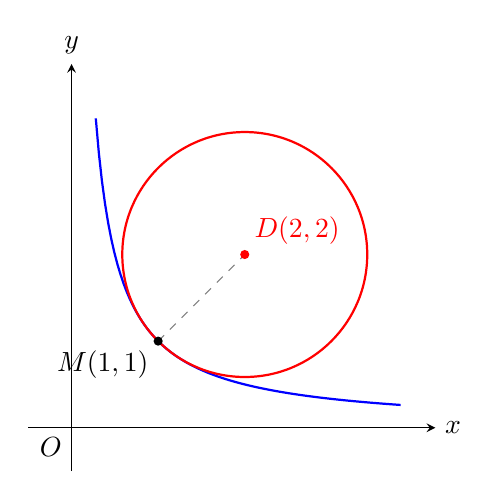
\begin{tikzpicture}[scale=1.1, >=stealth]
            \draw[->] (-0.5, 0) -- (4.2, 0) node[right] {$x$};
            \draw[->] (0, -0.5) -- (0, 4.2) node[above] {$y$};
            \node[below left] at (0, 0) {$O$};
            \begin{scope}
                \clip (-0.4, -0.4) rectangle (4, 4);
                \draw[thick, blue, domain=0.28:3.8, samples=100] plot (\x, {1/\x});
                \draw[red, thick] (2, 2) circle (1.414);
                \draw[dashed, gray] (1, 1) -- (2, 2);
            \end{scope}
            \fill (1, 1) circle (1.5pt) node[below left] {$M(1, 1)$};
            \fill[red] (2, 2) circle (1.5pt) node[above right] {$D(2, 2)$};
        \end{tikzpicture}
    \end{center}
    \begin{equation}
        \boxed{k = \frac{\sqrt{2}}{2}, \quad \rho = \sqrt{2}, \quad D(2, 2).}
    \end{equation}

    \ansitem{2}

    对 $y = \e^{-x^2}$ 求导：$y' = -2x\e^{-x^2}$，$y'' = (4x^2 - 2)\e^{-x^2}$．在点 $(0, 1)$ 处，$y' = 0$，$y'' = -2$．
    \begin{equation}
        k = \frac{|-2|}{(1 + 0)^{3/2}} = 2, \qquad \rho = \frac{1}{2},
    \end{equation}
    \begin{equation}
        \xi = 0 - 0 = 0, \qquad \eta = 1 + \frac{1}{-2} = \frac{1}{2}.
    \end{equation}
    \begin{equation}
        \boxed{k = 2, \quad \rho = \frac{1}{2}, \quad D\left(0, \frac{1}{2}\right).}
    \end{equation}
\end{solution}

\begin{problem}{参数方程曲线的曲率计算}{Curvature-Of-Parametric-Curves}
    求下列曲线在指定点的曲率：
    \begin{enumerate}
        \item $\begin{cases} x = 3t^2, \\ y = 3t - t^3 \end{cases}$ 在 $t = 1$ 处；
        \item $\begin{cases} x = \cos t + t\sin t, \\ y = \sin t - t\cos t \end{cases}$ 在 $t = \frac{\uppi}{2}$ 处．
    \end{enumerate}
\end{problem}

\begin{solution}
    参数方程曲率计算公式为
    \begin{equation}
        k = \frac{|\dot{x}\ddot{y} - \ddot{x}\dot{y}|}{(\dot{x}^2 + \dot{y}^2)^{3/2}}.
    \end{equation}

    \ansitem{1}

    计算各阶导数：
    \begin{equation}
        \dot{x} = 6t, \quad \ddot{x} = 6, \qquad \dot{y} = 3 - 3t^2, \quad \ddot{y} = -6t.
    \end{equation}
    在 $t = 1$ 处，$\dot{x} = 6, \ddot{x} = 6, \dot{y} = 0, \ddot{y} = -6$．代入得
    \begin{equation}
        k = \frac{|6(-6) - 6(0)|}{(6^2 + 0^2)^{3/2}} = \frac{36}{216} = \frac{1}{6}.
    \end{equation}
    \begin{equation}
        \boxed{k = \frac{1}{6}.}
    \end{equation}

    \ansitem{2}

    计算各阶导数：
    \begin{equation}
        \dot{x} = t\cos t, \quad \ddot{x} = \cos t - t\sin t, \qquad \dot{y} = t\sin t, \quad \ddot{y} = \sin t + t\cos t.
    \end{equation}
    由此可得
    \begin{equation}
        \dot{x}\ddot{y} - \ddot{x}\dot{y} = t^2, \qquad \dot{x}^2 + \dot{y}^2 = t^2.
    \end{equation}
    曲率公式为 $k = \frac{t^2}{t^3} = \frac{1}{t}$．在 $t = \frac{\uppi}{2}$ 处，
    \begin{equation}
        k = \frac{2}{\uppi}.
    \end{equation}
    \begin{equation}
        \boxed{k = \frac{2}{\uppi}.}
    \end{equation}
\end{solution}

\begin{problem}{对数曲线最小曲率半径的求解}{Minimum-Curvature-Radius-Of-Logarithmic-Curve}
    对数曲线 $y = \ln x$ 上哪一点的曲率半径最小？并求出该点的曲率半径．
\end{problem}

\begin{solution}
    对 $y = \ln x$（$x > 0$）求导：$y' = \frac{1}{x}$，$y'' = -\frac{1}{x^2}$．曲率半径为
    \begin{equation}
        \rho(x) = \frac{(1 + y'^2)^{3/2}}{|y''|} = \frac{\left( 1 + \frac{1}{x^2} \right)^{3/2}}{\frac{1}{x^2}} = \frac{(x^2 + 1)^{3/2}}{x}.
    \end{equation}
    为求极值，令 $u(x) = \ln \rho(x) = \frac{3}{2}\ln(x^2 + 1) - \ln x$．求导得
    \begin{equation}
        u'(x) = \frac{3x}{x^2 + 1} - \frac{1}{x} = \frac{2x^2 - 1}{x(x^2 + 1)}.
    \end{equation}
    令 $u'(x) = 0$，解得唯一驻点 $x = \frac{\sqrt{2}}{2}$．

    当 $x \in \left(0, \frac{\sqrt{2}}{2}\right)$ 时 $u'(x) < 0$；当 $x \in \left(\frac{\sqrt{2}}{2}, +\infty\right)$ 时 $u'(x) > 0$．

    故在点 $P\left( \frac{\sqrt{2}}{2}, -\frac{1}{2}\ln 2 \right)$ 处曲率半径取得全域最小值，最小值为
    \begin{equation}
        \rho\left(\frac{\sqrt{2}}{2}\right) = \frac{\left(\frac{1}{2} + 1\right)^{3/2}}{\frac{\sqrt{2}}{2}} = \frac{3\sqrt{3}}{2}.
    \end{equation}
    \begin{equation}
        \boxed{\text{在点 } \left( \frac{\sqrt{2}}{2}, -\frac{1}{2}\ln 2 \right) \text{ 处曲率半径最小，最小值为 } \frac{3\sqrt{3}}{2}.}
    \end{equation}
\end{solution}

\begin{problem}{全轴有界凸函数的常数性}{Bounded-Convex-Function-On-Real-Line}
    设函数 $f(x)$ 是定义在 $(-\infty, +\infty)$ 上的凸函数且有上界．求证：$f(x)$ 是常数．
\end{problem}

\begin{myproof}
    设存在常数 $M$，使得对任意 $x \in \symbb{R}$ 恒有 $f(x) \leqslant M$．

    任取两点 $x_1 < x_2$，考虑割线斜率 $k = \frac{f(x_2) - f(x_1)}{x_2 - x_1}$．

    若 $k > 0$，对任意 $x > x_2$，由凸函数的三割线斜率单调性，有
    \begin{equation}
        \frac{f(x) - f(x_2)}{x - x_2} \geqslant \frac{f(x_2) - f(x_1)}{x_2 - x_1} = k \implies f(x) \geqslant f(x_2) + k(x - x_2).
    \end{equation}
    在不等式两边令 $x \to +\infty$，得 $\lim_{x\to +\infty} f(x) = +\infty$，这与 $f(x)$ 有上界矛盾．

    若 $k < 0$，对任意 $x < x_1$，由凸函数的斜率单调性，有
    \begin{equation}
        \frac{f(x_1) - f(x)}{x_1 - x} \leqslant \frac{f(x_2) - f(x_1)}{x_2 - x_1} = k \implies f(x) \geqslant f(x_1) - k(x_1 - x).
    \end{equation}
    在不等式两边令 $x \to -\infty$，得 $\lim_{x\to -\infty} f(x) = +\infty$，同样与 $f(x)$ 有上界矛盾．

    因此必有 $k = 0$，即 $f(x_1) = f(x_2)$．

    由 $x_1, x_2$ 的任意性，函数 $f(x)$ 必恒为常数．
\end{myproof}

\endinput
